%%%%%%%%%%%%%%%%%%%%%%%%%%%%%%%%%%%%%%%%%%%%%%%%%%%%%%%%%%%%%%%%%%%%%%%%%%%%%%%%%%%%%%%%%%%%%%%%%%
\begin{frame}[label=ExistenciaMao,noframenumbering]
	\frametitle{Apendice A: Existencia y unicidad (condiciones locales)}    	
	\begin{overlayarea}{\textwidth}{1.0\textheight}	
	\begin{columns}
		\column{.57\textwidth}
			\begin{Teorema}
				 (EU-1)-(EU-3)	 			
	 			$\Rightarrow$ 
	 			$\exists ! \  \{y(t)\}_{t\geq 0}$, $\forall y(0)=y_0\in \mathbb{R}^d$. 
				\\				
				Adem\'as $0<T<\infty$,
				\begin{itemize}[<+-|alert@+>]
					\item				
					$
						\EX{y(T)}< 
							\left(
								|y_0|^2 +2\alpha T 
							\right)\exp(2\beta T),
					$
					\item				
					$\tau_n := \inf \{ t\geq 0 : |y(t)|>n\}$, $n\in \N$,					
					\only<3->{
						$$	
							\textcolor<3>{red}{
								\prob{[\tau_n\leq T]}
								\leq \frac{
								\left(
								|y_0|^2 +2\alpha T 
								\right)
								\exp(2\beta T)
								}{n},
							}
						$$ 
					}	
					\item<4>					
						$
							\textcolor<4>{red}{
								\EX{|y(t)|^p}
								\leq
								2^{\frac{p-2}{2}}
								\left(
								1 + \EX{|y_0|^p}
								\right)e^{Cpt}.				
							}
						$			
				\end{itemize}			
			\end{Teorema}
		\column{.5\textwidth}		
			\begin{bibunit}[apalike]		
				\cite{Mao2013}			
				\biblio{PhdThesisBib.bib}
			\end{bibunit}
	\end{columns}
		
	\hyperlink{Construccion<1>}{
		\beamerreturnbutton{Construcc\'on}
	}
	\end{overlayarea}
\end{frame}
%%%%%%%%%%%%%%%%%%%%%%%%%%%%%%%%%%%%%%%%%%%%%%%%%%%%%%%%%%%%%%%%%%%%%%%%%%%%%%%%%%%%%%%%%%%%%%%%%%
\begin{frame}[label=MatrixFunctions,noframenumbering]
	\frametitle{Apendice A}
	\scalebox{0.85}{\parbox{1.0\linewidth}{
		\begin{align*}	
			A^{(1)}(h,u)&:=
			\begin{pmatrix}
				e^{ha_1(u)} & \multicolumn{2}{c}{\text{\kern0.5em\smash{\raisebox{-1ex}{\huge 0}}}} \\
				&\ddots\\
				\multicolumn{2}{c}{\text{\kern-0.5em\smash{\raisebox{0.95ex}{\huge 0}}}} 
				& e^{ha_d(u)}
			\end{pmatrix},
			\\
		%	
			A^{(2)}(h,u)&:=
			\begin{pmatrix}
				\left(
					\displaystyle
					\frac{e^{ha_1(u)} - 1}{a_1(u)}
				\right)\1{E_1^c}	& 
				\multicolumn{2}{c}{\text{\kern0.5em\smash{\raisebox{-1ex}{\huge 0}}}}\\
				& \ddots&\\
				\multicolumn{2}{c}{\text{\kern0.5em\smash{\raisebox{-1ex}{\huge 0}}}}&
				\left(
					\displaystyle
					\frac{e^{ha_d(u)} - 1}{a_d(u)}
				\right)\1{E_d^c}% + h \1{E_i} 
			\end{pmatrix}
			+h
			\begin{pmatrix}
				\1{E_1} & \multicolumn{2}{c}{\text{\kern0.5em\smash{\raisebox{-1ex}{\huge 0}}}}\\
				&\ddots &\\
				\multicolumn{2}{c}{\text{\kern0.5em\smash{\raisebox{-1ex}{\huge 0}}}} &
				\1{E_d}
			\end{pmatrix},\\	
			E_j&:=\{x \in \R^d: a_j(x)=0\} , \qquad 
			b(u):= 
			\left(
				b_1(u^{(-1)}), \dots , b_d(u^{(-d)})
			\right)^T.		
		\end{align*}
		}
	}
	\\
	\hyperlink{Construccion<6>}{\beamerreturnbutton{Teorema}}
\end{frame}
%%%%%%%%%%%%%%%%%%%%%%%%%%%%%%%%%%%%%%%%%%%%%%%%%%%%%%%%%%%%%%%%%%%%%%%%%%%%%%%%%%%%%%%%%%%%%%%%%%
\begin{frame}[label=ZerosConditions, noframenumbering]
	\frametitle{Apendice B: Resultato para ceros no aislados}    
	\begin{columns}
		\column{.6\textwidth}
			\begin{Teorema}[L'h\^{o}pital Multivariable] 
				\begin{itemize}
					\item 
						$\mathcal{N}$ vecindad en $\R^2$ de $\mathbf{p}$ donde
						$f:\mathcal{N}\to \R$,  
						$g:\mathcal{N}\to \R$ diferenciables son cero. 
					\item
						$
							C=\{x \in \mathcal{N}: f(x)=g(x)=0 \},
						$				
					\item
						Supón $C$ suave, que pasa por $\mathbf{p}$.
					\item
					 $\exists \ \mathbf{v}$ no tangente a $C$ en $\mathbf{p}$
						t.q  $D_{\mathbf{v}}g$ en la dirección $\mathbf{v}$ es no nula en
						$\mathcal{N}$.
					\item
						$\mathbf{p}$ es punto limite de $\mathcal{N}\setminus C$. 
			\end{itemize}
	    Entonces
				$
					\displaystyle
					\lim_{(x,y)\to \mathbf{p}}
					\frac{f(x,y)}{g(x,y)} =
					\lim_{
						\substack{
							(x,y)\to \mathbf{p}\\ 
							(x,y)\in \mathcal{N} \setminus C
						}
					}
					\frac{D_{\mathbf{v}} f }{D_{\mathbf{v}} g},
				$
				siempre que exista el limite.
			\end{Teorema}
			\column{.4\textwidth}
				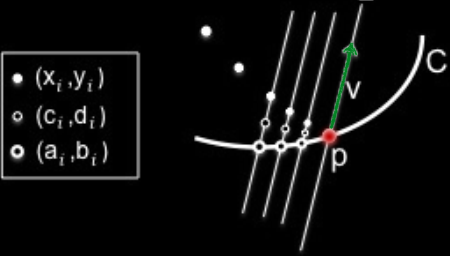
\includegraphics[width=\linewidth]{Imagenes/Apendice/LawlorThm.png}
				\\
				\hyperlink{Construccion<6>}{\beamerreturnbutton{Hip\'otesis}}
				\begin{bibunit}[alpha]
					\nocite{Lawlor2012}
					\biblio{PhdThesisBib.bib}
				\end{bibunit}
	\end{columns}
\end{frame}
%%%%%%%%%%%%%%%%%%%%%%%%%%%%%%%%%%%%%%%%%%%%%%%%%%%%%%%%%%%%%%%%%%%%%%%%%%%%%%%%%%%%%%%%%%%%%%%%
\begin{frame}[noframenumbering]
	\frametitle{Apendice B: Resultado para ceros aislados}    
	\begin{columns}
		\column{.4\textwidth}
		\begin{definicion}[DD respecto a $p$]
			 $u,\mathbf{p}\in \R^2$,  $\alpha$ angulo positivo respecto a eje-$x$ 
			segmento $\overline{u \mathbf{p}}$.	 
			\begin{align*}
				f_{\alpha}(u) &= 
				\frac{ \innerprod{q-u}{\nabla f(u)}}{|u-q|}			
			\end{align*}
			 \emph{derivada direccional respecto $\mathbf{p}$ en $u$}.
		\end{definicion}
		\begin{definicion}[Star-like set]
			$S\subset \R^2$ es \emph{star-like} respecto $\mathbf{p}$,  $\forall \ s \in S$ 
			el segmento abierto	$\overline{s \mathbf{p}}$  esta en $S$.
		\end{definicion}

		\column{.6\textwidth}
		%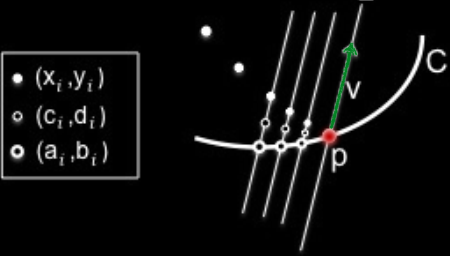
\includegraphics[width=\linewidth]{Imagenes/Apendice/LawlorThm.png}
		\begin{Teorema}
			\begin{itemize}
				\item 
					$\mathbf{p}\in \R^2$, $S\subset \R^2$ star-like respecto $\mathbf{p}$ en el dominio de $f$,$g$.
				\item
					En $S$, $f,g$ diferenciables , $g_{\alpha}(s)\neq 0$, 	
				\item 
					$f(\mathbf{p})=g(\mathbf{p})=0$,
					\quad
					$
						\displaystyle
						\lim_{x \to \mathbf{p}}
						\frac{f_{\alpha}(x)}{g_{\alpha}(x)} = L,	
					$
			\end{itemize}
			Entonces
				$ 
					\displaystyle
					\lim_{x \to \mathbf{p}}
					\frac{f(x)}{g(x)} = L.
				$
		\end{Teorema}
		\begin{bibunit}[alpha]
			\nocite{FineAIandKass1966}
			\biblio{PhdThesisBib.bib}
		\end{bibunit}
	\end{columns}
\end{frame}
%%%%%%%%%%%%%%%%%%%%%%%%%%%%%%%%%%%%%%%%%%%%%%%%%%%%%%%%%%%%%%%%%%%%%%%%%%%%%%%%%%%%%%%%%%%%%%%%
\begin{frame}[noframenumbering]
	\frametitle{Apendice B: Condiciones para ceros de $a_j(\cdot)$}    
		\textcolor{orange}{
			 $E_j:=\{x\in \R^{d}: a_j(x)=0\}$
		} satisface alguno de los puntos:
		\begin{enumerate}[(i)]
			\item
				 $p \in E_j$ es un cero no aislado de  $a_j(\cdot)$ y:
			\begin{itemize}
				\item  
					\textcolor{cyan}{
					$
						D:=\{u: e^{ha_j(u)}-1=a_j(u)= 0\},
					$ 
				}
				es una curva suave que pasa por $p$. 
				\item
				El vector canónico $e_j$ es no tangente a $D$.
				\item
					Para cada $p \in E_j$, existe una bola $B_r(p)$ t.q.
				$$
					a_j\neq 0, \qquad
					\frac{\partial a_j(u)}{\partial u^{(j)}} \neq 0 ,\qquad 
					\forall u \in D
					\setminus B_r(p).
				$$
			\end{itemize}	
			\item
				 $p \in E_j$ es un cero aislado de $a_j(\cdot)$ y:
			\begin{itemize}
				\item
					Para cada $q\in E_j$,  $p$ no es punto limite de
					$E_{\alpha}:=\{x \in \R^d: (a_j)_\alpha(x)=0\}$.
				\item
					Para cada $p \in E_j$ existe  $B_r(p)$, t.q.
					la derivada direccional respecto a $p$ satiface
				$$
				(a_j)_\alpha(x) \neq 0, \qquad \forall x\in B_r(p).
				$$
			\end{itemize}		
		\end{enumerate}
\end{frame}
